\section{Background}
\label{background}

\subsection{Research area}
\label{research_area}
%What is the research area?
Many applications use algorithms to find distances between data points in a (typically large) data set in order to extract knowledge based on this. 
%TODO: Specifik reference/eksempel
One example is doing similarity search, or more specifically nearest-neighbor (NN) search, on pictures to recognize letters or numbers. As useful as this is, it still depends on the given data, which are getting increasingly big in size. This is a general problem as even modern machines are not able to process \textit{gigantic} files all at once(i.e. keeping all the data in main memory). Thus another big subject in computer science arises, that is compressing the data in order to fit in memory while trying to preserve as many properties from the data as possible. This research area is what \qs{} deals with, and in particular for high-dimensional data sets.
\\
\\
Naturally one must pay to compress something, which happens in terms of accuracy, i.e. representing the data using only approximations. This also means that there is a trade off between compression and accuracy for the algorithms in this area. That is why compression algorithms usually are measured on these parameters, i.e. accuracy per compression size.
\\
\\
Distance preserving compression algorithms are usually divided into two categories: data-oblivious and data-dependent. The former attempts to achieve guarantees for any data set while the latter attempts to use the extra information about the particular data sets in order to design functions with better performance. Compressed representations makes computation for data analysis algorithms more efficient, which is very desirable in many fields, such as data mining and machine learning.\cite{stan15}

\subsection{The \qs{} compression scheme}
\label{qs}
The sketch is a compressed representation of a point set \texttt{X}. The points of \texttt{X} have \texttt{d} dimensions and are in \textit{euclidean} space. Each coordinate of a point is represented by \texttt{B} bits implying a point is represented by \textit{dB} bits. \qs{} will take as input the point set \texttt{X} and two additional parameters \texttt{L} and $\Lambda$. These two parameters are used to specify the compression of the point set where \texttt{L} is the depth of the \qt{} and $\Lambda$ is the amount of nodes from the \qt{} which can be removed. 
%TODO: PRÆCISÉR parametre
There are three steps for building the sketch: randomly shifted grid, \qt{} construction and pruning. These steps will be explained briefly and there will be given an example of how a sketch is built on a small example.
\\
\\
The first step is randomly shifted grid. Here there is constructed a hypercube \texttt{H} which contains all points of the given point set \texttt{X}. \texttt{H} will then be set up to be centered around a point of \texttt{X}. Then choose a random value $\sigma$ for each dimension of the hypercube. For each dimension \texttt{j} of \texttt{H} will be shifted with $\sigma_j$.
\\
\\
The next step is creating the \qt{}. A \textit{2d-ary} \qt{} is created by starting at the root of \texttt{H}. There is then only added the children which contain a point from \texttt{X}, thus child nodes that do not contain a point from \texttt{X} are ignored. Each edge to a child node is labeled with a \textit{d} long bit string that has been split on. This step is then done recursively until the level \texttt{L} is reached. An example of a constructed \qt{} is given in figure \ref{fig:quadtree}.

%TODO: SÆT STØRRELSEN OP MAND!!!
\begin{figure}
	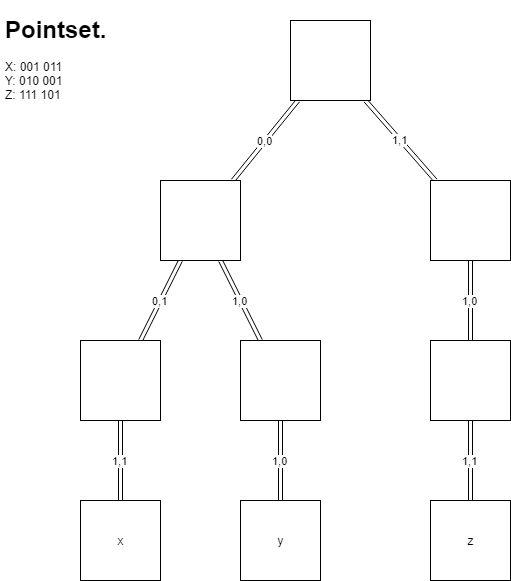
\includegraphics[width=0.5\textwidth]{figures/quadtree}
	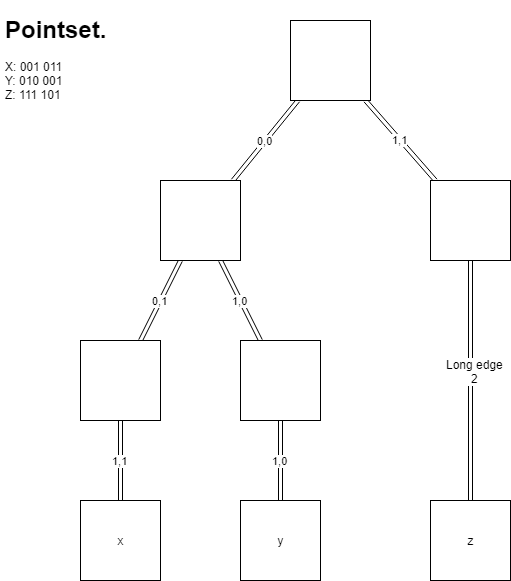
\includegraphics[width=0.5\textwidth]{figures/prunnedquadtree}
	\caption{On the left there is shown the \qt{} after construction with $L=4$. On the right the \qt{} has been pruned with a $\Lambda = 1$}
	\label{fig:quadtree}
\end{figure}

After construction of the \qt{} the tree is pruned. There are found downward paths $n_0,...,n_k$ where nodes $n_1,...,n_{k-1}$ all have a degree 1. If \ensuremath{\texttt{k} > \Lambda+1} then there are removed nodes $n_{\Lambda+1},...,n_{k-1}$ from the \qt{}. Instead node $n_{\Lambda}$ is connected directly to $n_{k}$ with an edge. This edge is called a long edge and is labeled with the length of the path it replaces. This is given an example of the tree after a pruning in figure \ref{fig:quadtree}.


From this the sketch can be built. There is used the "Eulerian Tour Technique"\footnote{See e.g., \url{https://en.wikipedia.org/wiki/Euler\_tour\_technique}}.
It starts at the root an searches down to the leftmost leaf. It will then back track up to its parents until it finds an new leaf it can traverse down to. When an edge is explored downwards there is stored a 0 and the label of the edge either a bit string or the length of an long edge. Also for each downward movement there is stored a bit specifying if the given edge is a long or short edge. If an upwards edge is explored then a 1 is stored. Furthermore, there is stored for each point an index for the child node which contains it.
%TODO: Review this subsection to properly and precisely describe QS

\subsection{Related work}
\label{state_of_the_art}
Several state of the art algorithms exist for the research area introduced in section \ref{research_area}. \cite{wagner17} mentions \textit{Product Quantization} (\pq{}), which they use as reference state of the art algorithm in their experiments. The \pq{} concept is stated in its original paper, \cite{schmid9}, as such "The idea is to decomposes the space into a Cartesian product of low dimensional subspaces and to quantize each subspace separately", where the term \textit{quantize} refers to the process of constraining an input from a continuous set of values to a discrete set\footnote{E.g. real numbers to integers. See https://en.wikipedia.org/wiki/Quantization 11-04-2018}.

Well known general algorithms and data structures exists for the same purpose, such as \textit{k-means} and \textit{kd-trees}, where the former is a clustering algorithm and the latter is an adaptive data structure for spatial data sets. This is also discussed in \cite{schmid9}, where it is noted that apparently a pure brute-force algorithm outperforms these in practice for high-dimensional data. Further algorithms listed in this paper include "spectral hashing"\cite{weiss8}, "Hamming embedding"\cite{jegou8}, and "FLANN"\cite{muja9}. These will not be investigated further, but are only mentioned for reference.
%TODO: Elaborate on closely related work and insert citations

%From ILO:
%"Identify and formulate precisely (if possible) the algorithmic problem hidden in a given programming task."